\documentclass{beamer}
\usepackage[utf8]{inputenc}

\usepackage{utopia} %font utopia imported
% \usepackage{caption}
% \captionsetup{font=scriptsize,labelfont=scriptsize}

\setbeamerfont{caption}{series=\normalfont,size=\fontsize{8}{10}}

\usetheme{Madrid}
\usecolortheme{default}

\definecolor{RedCIMAT}{rgb}{0.44921875, 0.13671875, 0.234375} % UBC Blue (primary)
\usecolortheme[named=RedCIMAT]{structure}

\setbeamertemplate{caption}[numbered]

\newcommand\Fontvi{\fontsize{10}{12.2}\selectfont}
\newcommand\FontEq{\fontsize{8}{12.2}\selectfont}

%------------------------------------------------------------
%This block of code defines the information to appear in the
%Title page
\title[Avance de Tesis] %optional
{Métodos de Análisis de Secuencias basados en Aprendizaje Profundo en problemas de Visión y Procesamiento de Imágenes}

\subtitle{Estimación de Pose y Clasificación de Imágenes}

\author[Esaú Peralta] % (optional)
{Óscar Esaú Peralta Rosales\inst{1} \and Dr. Mariano Rivera Meraz\inst{1}}

\institute[CIMAT] % (optional)
{
  \inst{1}%
  Centro de Investigación en Matemáticas A.C.
}

\date[Julio 2021] % (optional)
{Avance de Tesis}

\logo{
\includegraphics[height=0.7cm]{logo.jpg}}
%End of title page configuration block
%------------------------------------------------------------



%------------------------------------------------------------
%The next block of commands puts the table of contents at the
%beginning of each section and highlights the current section:

\AtBeginSection[]
{
  \begin{frame}
    \frametitle{Table of Contents}
    \tableofcontents[currentsection]
  \end{frame}
}
%------------------------------------------------------------


\begin{document}

%The next statement creates the title page.
\frame{\titlepage}


%---------------------------------------------------------
%This block of code is for the table of contents after
%the title page
\begin{frame}
\frametitle{Tabla de Contenido}
\tableofcontents
\end{frame}
%---------------------------------------------------------


\section{Motivación de la Tesis}


%---------------------------------------------------------
%Changing visibility of the text
\begin{frame}
\frametitle{Motivación de la Tesis}
Con el auge de los Transformes como modelos de procesamiento de información secuencial, el trabajo
de esta tesis ha sido dirigido en explorar dichos modelos en áreas fuera del Procesamiento del
Lenguaje Natural.\\~\

Finalmente se propone una variante enfocado en aumentar la capacidad receptiva de las cabezas de
atención permitiendo mayor flexibilidad al no estar ligada al tamaño de embedding predefinidos.\\~\

Las experimentaciones del funcionamiento la variante del modelo se realizan en los siguientes
problemas:
\begin{itemize}
    \item Predicción de Pose 2D en humanos sobre imágenes
    \item Predicción de Pose 3D en humanos (Monocular, Desacoplado)
    \item ViT y Clasificación de Enfermedades Comunes de Tórax (INAOE, CIMAT, IMSS)
\end{itemize}
\end{frame}

%---------------------------------------------------------

\section{Descripción de los Problemas}

%---------------------------------------------------------
%Highlighting text
\begin{frame}
\frametitle{Estimación de Pose 2D y 3D en Humanos}

\begin{itemize}
    \item 2D: Dada una imágen estimar las posiciones de las articulaciones de la persona en cuestión
          sobre la imagen.
    \item 3D: Dada una imagen estimar las posiciones de las articulaciones dentro de un marco de
          referencia que mejor ajuste la posición espacial de la persona en cuestión.
\end{itemize}

\begin{columns}
\column{0.5\textwidth}
\begin{figure}[htbp]
    \centerline{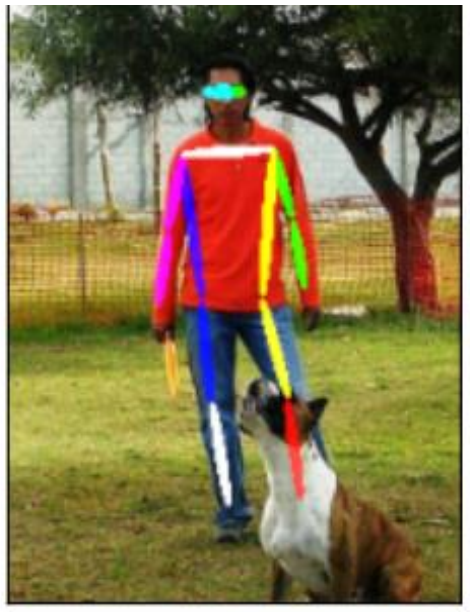
\includegraphics[height=1in]{images/example_2D.png}}
    \caption{Estimación de Pose 2D}
    \label{fig:ie2d}
\end{figure}

\column{0.6\textwidth}
\begin{figure}[htbp]
    \centerline{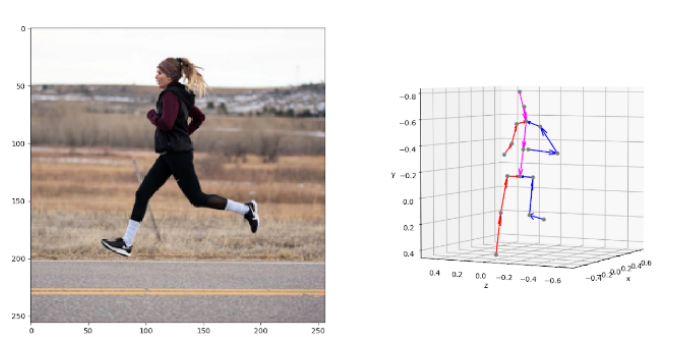
\includegraphics[height=1in]{images/example_3D.png}}
    \caption{Estimación de Pose 3D}
    \label{fig:ie3d}
\end{figure}
\end{columns}
\end{frame}
%---------------------------------------------------------


%---------------------------------------------------------
%Two columns
\begin{frame}
\frametitle{Estimación de Pose 2D y 3D en Humanos}

\begin{columns}

\column{0.4\textwidth}
Esqueleto
\begin{itemize}
    \item 17 articulaciones
    \item 16 huesos \\~\
\end{itemize}

Datasets
\begin{itemize}
    \item Human 3.6M
    \item COCO 2017
\end{itemize}

\column{0.6\textwidth}
\begin{figure}[htbp]
    \centerline{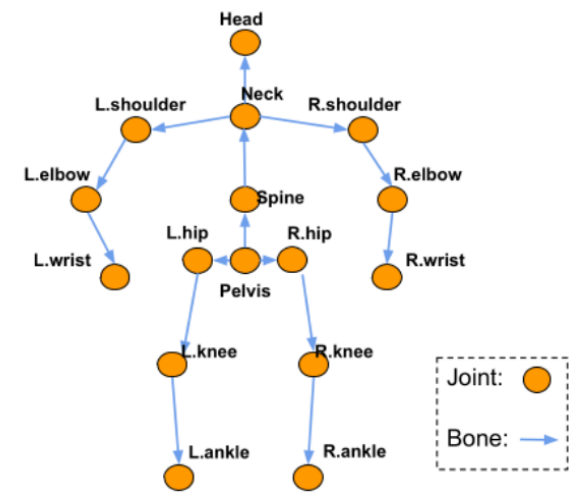
\includegraphics[height=1.5in]{images/joints.png}}
    \caption{Articulaciones usadas en tareas de Estimación de Pose en Humanos. Imagen tomada del
    artículo "Anatomy-Aware 3D Human Pose Estimación en Videos"}
    \label{fig:joints}
\end{figure}

\end{columns}

\end{frame}
%---------------------------------------------------------

%---------------------------------------------------------
%Two columns
\begin{frame}
\frametitle{Detección y Clasificación de Enfermedades Comunes de Tórax}

% La examinación por Rayos-X es uno de los métodos más comunes para la detección y diagnóstico de
% enfermedades que atacan la zona toráxica.

\begin{columns}
\column{0.5\textwidth}
\begin{itemize}
    \item Trabajo colaborativo entre CIMAT, INAOE e IMSS.
    \item Modelo clasificador para la detección de 15
          padecimientos incluyendo COVID-19.
    \item Se realiza la comparativa de un modelo basado en ViT con las modificaciones antes
          mencionadas.
\end{itemize}

\column{0.5\textwidth}
\begin{figure}[htbp]
    \centerline{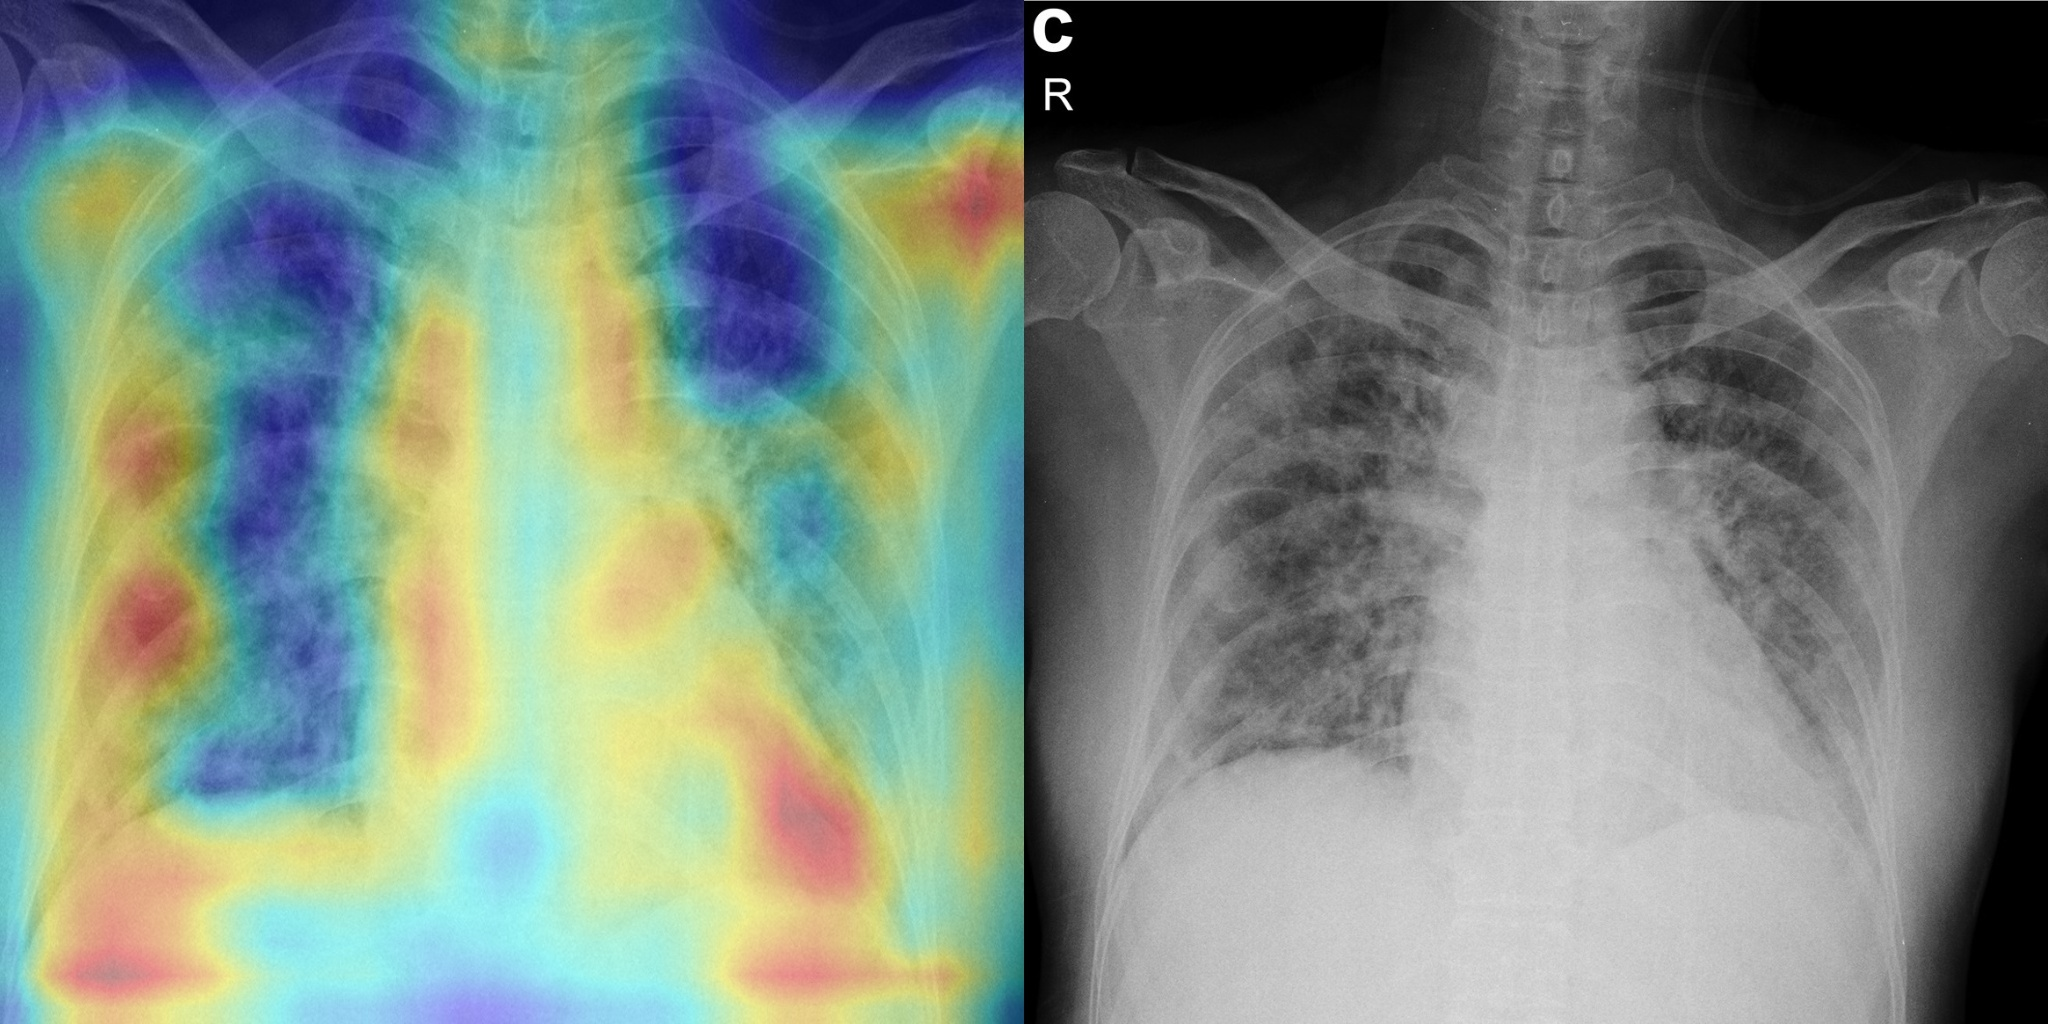
\includegraphics[width=1.5in]{images/lung_covid.jpg}}
    \caption{Áreas Afectadas por COVID-2019 detectadas por el modelo usando GradCam.}
    \label{fig:lung}
\end{figure}
\end{columns}

\end{frame}
%---------------------------------------------------------

\section{Modelos}

%---------------------------------------------------------
\begin{frame}
\frametitle{Modelo Estimación de Pose 2D}

\begin{figure}[htbp]
    \centerline{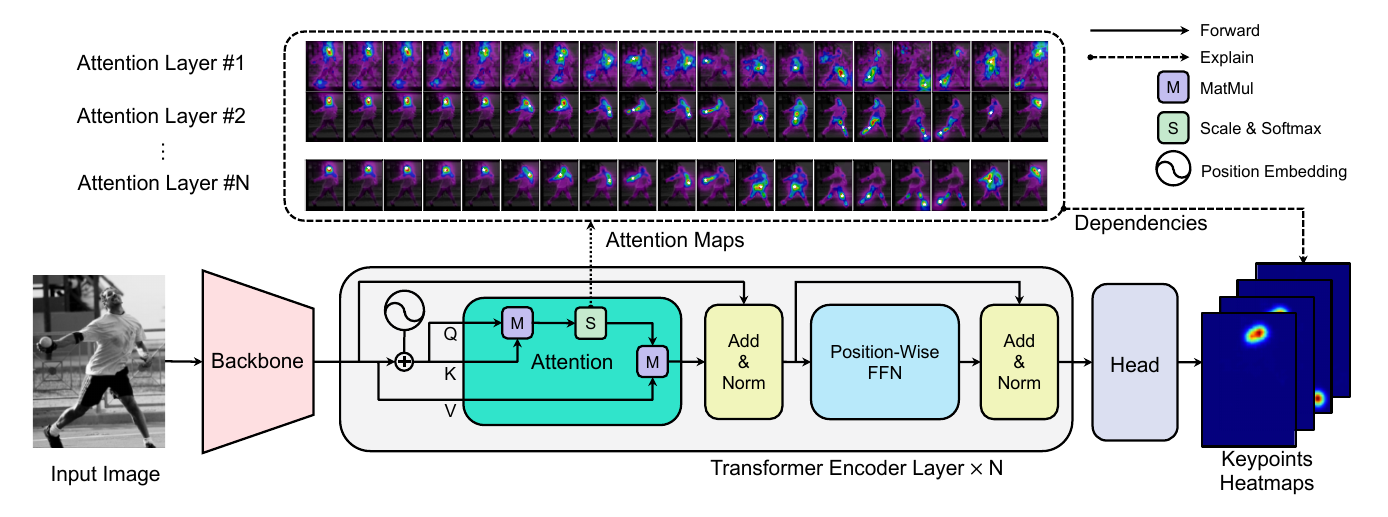
\includegraphics[width=5.0in]{images/model_2D.png}}
    \caption{Modelo Predicción de Pose 2D. Al igual que ViT usa capas con Decoders con entrada las
             características obtenidas por un modelo convolucional usado como Backbone}
    \label{fig:m2d}
\end{figure}

\end{frame}
%---------------------------------------------------------

%---------------------------------------------------------
\begin{frame}
\frametitle{Modelo Estimación de Pose 3D y ViT}
\begin{columns}
\column{0.4\textwidth}
    \begin{figure}[htbp]
        \centerline{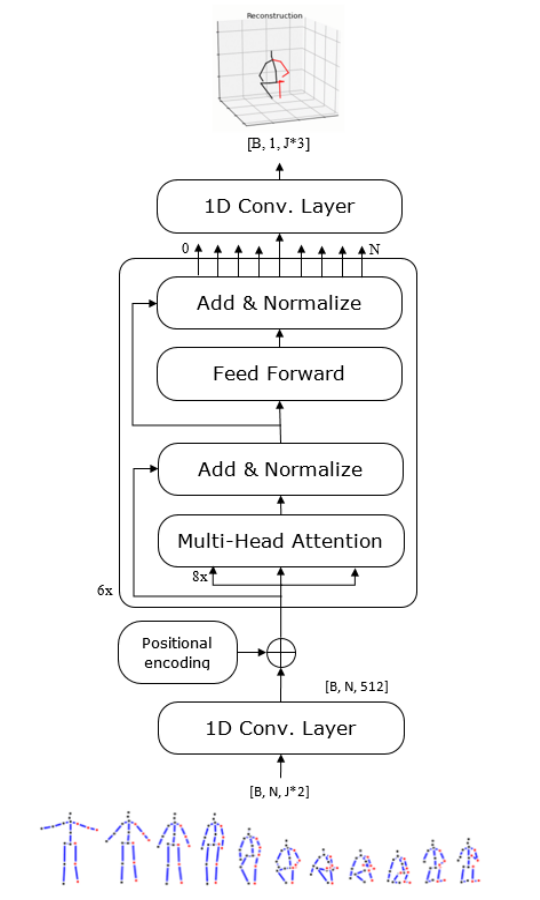
\includegraphics[height=2.1in]{images/model_3D.png}}
        \caption{Modelo Estimación de Pose 3D. Solo usa capas con Decoders.}
        \label{fig:m3d}
    \end{figure}

\column{0.6\textwidth}
    \begin{figure}[htbp]
    \centerline{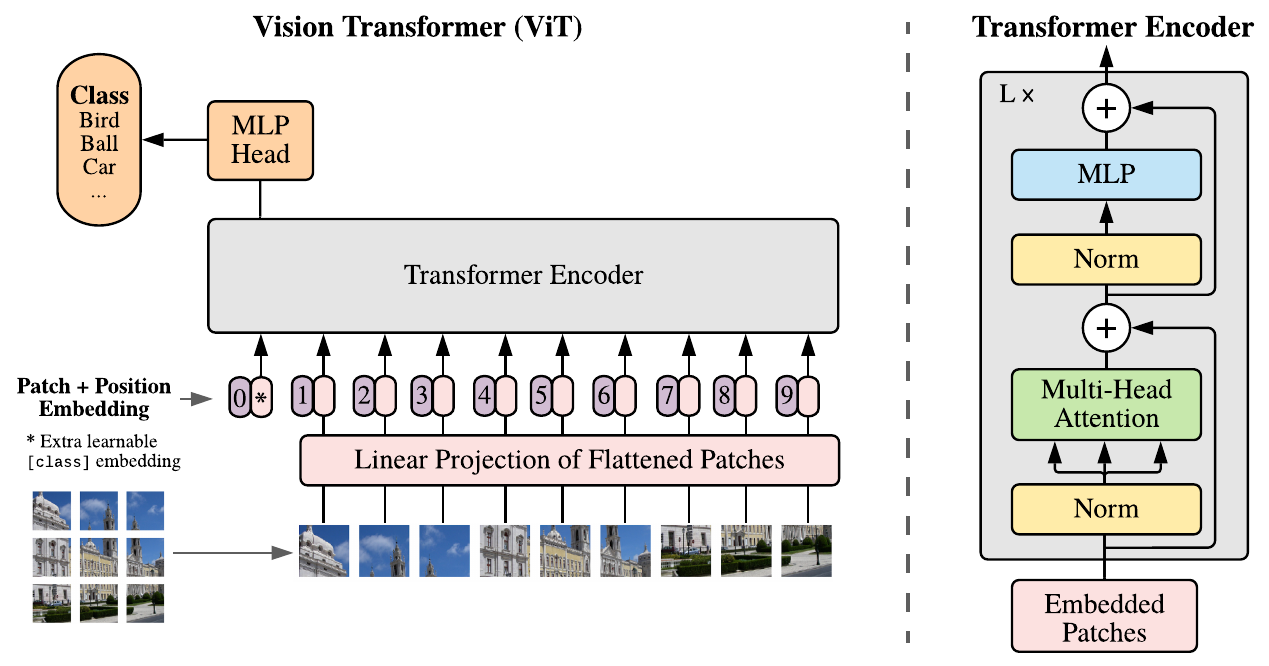
\includegraphics[width=2.5in]{images/model_vit.png}}
    \caption{Modelo ViT usado en las tareas de clasificación de enfermedades
             pulmonares. La entrada es una secuencia obtenida al dividir la imagen
             en pequeños parches.}
    \label{fig:vit}
    \end{figure}
\end{columns}

\end{frame}
%---------------------------------------------------------

%---------------------------------------------------------
% \begin{frame}
% \frametitle{Modelo Estimación de Pose 3D}

% \begin{figure}[htbp]
%     \centerline{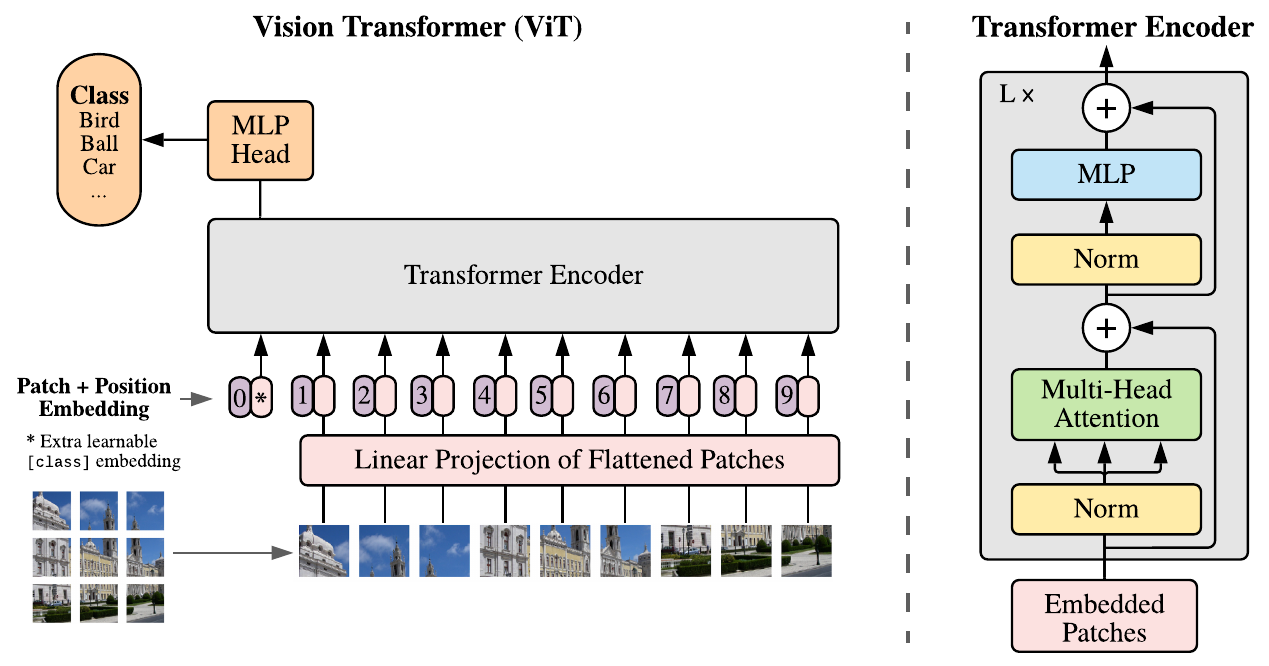
\includegraphics[height=2.0in]{images/model_vit.png}}
%     \caption{Modelo ViT usado en las tareas de clasificación de enfermedades
%              pulmonares. La entrada es una secuencia obtenida al dividir la imagen
%              en pequeños parches.}
%     \label{fig:vit}
% \end{figure}

% \end{frame}
%---------------------------------------------------------

\section{Variación a Transformes: Cabezas de Atención Flexibles}

%---------------------------------------------------------
\begin{frame}
\frametitle{MultiHead-Self-Attention}

\Fontvi
El Transformer está basado en la idea de Multihead-Self-Attention (MHA), permitiendo al modelo
conjuntamente atender a información en diferentes posiciones desde diferentes subespacios de
representación.

\FontEq
\begin{equation}
    mha(Q, K, V) = Concat(head_1,head_2,head_3,..., head_h)W^O
\end{equation}

\Fontvi
donde $Q, K, V \in \mathbb{R}^{n \times d_{m}}$ son embeddings de entrada, $n$ es el tamaño de la
secuencia, $d_m$ es el tamaño del embedding y $h$ el número de cabezas de atención. Cada cabeza es
definida como sigue:

\FontEq
\begin{equation}
    head_i = Attention(QW_i^Q, KW_i^K, VW_i^V) =
    Sofmax\Big(\frac{QW_i^Q (KW_i^K)^T}{\sqrt{d_k}}\Big) VW_i^V
\end{equation}

\Fontvi
donde $W_i^Q$, $W_i^K$ $\in \mathbb{R}^{d_m \times d_k}$, $W_i^V$ $\in \mathbb{R}^{d_m \times d_v}$,
$W^O$ $\in \mathbb{R}^{hd_v \times d_m}$ y $d_k=d_v=d_m/h$

\end{frame}
%---------------------------------------------------------

%---------------------------------------------------------
\begin{frame}
\frametitle{MultiHead-Self-Attention - Flexible}

\begin{itemize}
    \item El tamaño de la cabeza es dependiente de la dimensión del embedding y el número de cabezas
          de atención.
    \item Mientras más cabezas de atención los embeddings son proyectados a dimensiones cada vez
          más bajas, lo que implica una mayor compresión y perdida de información.
    \item Escalar el modelo implica escalar conjuntamente todas las dimensiones.\\~\
\end{itemize}

Redefiniendo  $W_i^Q$, $W_i^K$, $W_i^V$ $\in \mathbb{R}^{d_m \times d_h}$,
$W^O$ $\in \mathbb{R}^{hd_h \times d_m}$ con $d_h$ como un hiperparámetro y $d_h > d_k$
podemos solventar los puntos anteriores.

\end{frame}
%---------------------------------------------------------

\section{Resultados}

%---------------------------------------------------------
\begin{frame}
\frametitle{Detección de Pose 2D y 3D}

\tiny

\begin{table}
    \begin{center}
    \begin{tabular}{| c | c | c | c | c |}
        \hline
        \textbf{Modelo} & \textbf{$d_m$} & \textbf{$d_h$} & \textbf{AP} & \textbf{AR} \\
        \hline
        \hline
        Base & 256 & 32 & 0.726 & 0.780 \\
        \hline
        \hline
        Propio & 256 & 16 & 0.737 & 0.766 \\
        \hline
        Propio & 256 & 32 & 0.741 & 0.771 \\
        \hline
        Propio & 256 & 48 & 0.748 & 0.776 \\
        \hline
        \hline
        Propio $Q=K$ & 256 & 64 & 0.748 & 0.776 \\
        \hline
    \end{tabular}
    \end{center}
\caption{Average Precision y Average Recall sobre el conjunto de validación COCO-2017 para
         Estimación de Pose 2D.}
\label{table:2d}
\end{table}

\begin{table}
    \begin{center}
    \begin{tabular}{| c | c | c | c | c |}
        \hline
        \textbf{Modelo} & \textbf{$d_m$} & \textbf{$d_h$} & \textbf{Prot. 1} & \textbf{Prot. 2} \\
        \hline
        \hline
        Base & 512 & 64 & 37.7mm & 27.6mm \\
        \hline
        \hline
        Propio & 512 & 32 & 46.2mm & 33.7mm \\
        \hline
        Propio & 512 & 64 & 45.15mm & 32.96mm \\
        \hline
        Propio & 512 & 128 & 45.11mm & 32.84mm \\
        \hline
    \end{tabular}
    \end{center}
\caption{Error en milímetros usando Protocolos 1 y 2 para Estimación de Pose 3D.}
\label{table:3d}
\end{table}

\end{frame}
%---------------------------------------------------------

%---------------------------------------------------------
% \begin{frame}
% \frametitle{Detección de Pose 2D}
% \tiny
% \begin{table}[h!]
% \centering
% \begin{tabular}{|l||c|c|c|c|c|}
%     \hline
% {\bf Phatology} 		&	\multicolumn{4}{c|}{\bf Proposal}& CheXNeXt  \\
% \cline{2-5}
%                             &	PR AUC	&	ROC AUC	& F1-Score  & Accuracy  &  Accuracy \\
% \hline \hline
%     Cardiomegaly        	&	0.3003	&	0.8694	&	0.3196	&	0.8894	&	0.831	\\
%     Emphysema           	&	0.4014	&	0.9311	&	0.3317	&	0.8621	&	0.704	\\
%     Effusion            	&	0.4933	&	0.8336	&	0.5213	&	0.7606	&	0.901	\\
%     Hernia              	&	0.0499	&	0.8556	&	0.0514	&	0.9511	&	0.851	\\
%     Infiltration        	&	0.3863	&	0.7120	&	0.4656	&	0.6570	&	0.721	\\
%     Mass                	&	0.2886	&	0.8183	&	0.3293	&	0.8447	&	0.909	\\
%     Nodule              	&	0.2544	&	0.7951	&	0.2948	&	0.8509	&	0.894	\\
%     Atelectasis         	&	0.3400	&	0.7731	&	0.3882	&	0.7939	&	0.862	\\
%     Pneumothorax        	&	0.4422	&	0.8954	&	0.4954	&	0.8361	&	0.944	\\
%     Pleural-Thick.   	    &	0.1551	&	0.8033	&	0.2092	&	0.8130	&	0.798	\\
%     Pneumonia           	&	0.4248	&	0.8559	&	0.2802	&	0.8487	&	0.851	\\
%     Fibrosis            	&	0.1100	&	0.8540	&	0.1552	&	0.8971	&	0.806	\\
%     Edema               	&	0.1792	&	0.8657	&	0.1805	&	0.7330	&	0.924	\\
%     Consolidation       	&	0.1479	&	0.7519	&	0.2265	&	0.6813	&	0.893	\\
%     \hline
%     COVID-19            	&	0.8894	&	0.9987	&	0.8218	&	0.9987	&	---     \\
%     Healthy              	&	0.6897	&	0.7314	&	0.4829	&	0.7079	&	---	    \\
% \hline\hline
%     Average	            &	0.324	&	0.841	&	0.338	&	0.828	&	0.859	\\
% \hline
% \end{tabular}
% \caption{Resultados del modelo propuesto comparado con ChesXNeXt}
% \label{table_results_relabeled}
% \end{table}

% \end{frame}
%---------------------------------------------------------

%---------------------------------------------------------
\begin{frame}
\frametitle{Detección y clasificación de Enfermedades Comunes de Tórax}

\tiny

\begin{table}[h!]
\centering
\begin{tabular}{|l||c|c|c|c|c|r|}
    \hline
    \multicolumn{1}{|c||}{}	&	\multicolumn{4}{c|}{\bf Compared Models}    &	\multicolumn{2}{c|}{\bf Proposal} 	\\
    \cline{2-7}
                        &	CheXNeXt	&	CRAL	&	DR-CNN	&	TSNC    & Original	& Relabeled \\
\hline\hline
    Cardiomegaly        	&	0.885	&	0.880	&	0.801	&	0.887	& 0.869    &	0.920	\\
    Emphysema           	&	0.906	&	0.908	&	0.773	&	0.930	& 0.931	   &	0.959	\\
    Effusion            	&	0.825	&	0.829	&	0.797	&	0.831	& 0.834	   &	0.903	\\
    Hernia              	&	0.901	&	0.917	&	0.748	&   0.921   & 0.856	   &    0.961	\\
    Infiltration        	&	0.694	&	0.702	&	0.751	&	0.703	& 0.712	   &	0.817	\\
    Mass                	&	0.824	&	0.834	&	0.760	&	0.833	& 0.818	   &	0.874	\\
    Nodule              	&	0.759	&	0.773	&	0.741	&	0.798	& 0.795	   &	0.880	\\
    Atelectasis         	&	0.769	&	0.781	&	0.766	&	0.785	& 0.773	   &	0.859	\\
    Pneumothorax        	&	0.715	&	0.729	&	0.778	&	0.731	& 0.895	   &	0.949	\\
    Pleural-Thick.      	&	0.766	&	0.778	&	0.759	&	0.782	& 0.803	   &	0.913	\\
    Pneumonia           	&	0.852	&	0.857	&	0.800	&	0.881	& 0.856	   &	0.925	\\
    Fibrosis            	&	0.821	&	0.830	&	0.765	&	0.833	& 0.854	   &	0.943	\\
    Edema               	&	0.842	&	0.850	&	0.820	&	0.849	& 0.866	   &	0.949	\\
    Consolidation       	&	0.745	&	0.754	&	0.787	&	0.754	& 0.752	   &	0.886	\\
\hline
    COVID-19            	&	---	    &	--- 	&	---	    &	--- 	& 0.999    &	0.999	\\
    Healthy              	&	--- 	&	---	    &	--- 	&	---	    & 0.731    &	0.873	\\
\hline\hline
Average-14	            &	0.807	&	0.816	&	0.775	&	0.823	& 0.834	&	0.915	\\
Average	                &	---	    &	---	    &	---	    & 	---     & 0.841	&	0.916	\\
\hline
\end{tabular}
\caption{Comparativa de ROC AUC para distintos modelos sobre el conjunto de validación.}
\label{table_roc_auc_relabled}
\end{table}

\end{frame}
%---------------------------------------------------------

%---------------------------------------------------------
\begin{frame}
    \frametitle{Cronograma de Actividades Restantes}
    \begin{figure}[htbp]
        \centerline{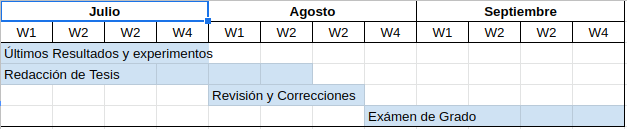
\includegraphics[height=1in]{images/crono.png}}
        \caption{Cronograma de Actividades}
        \label{fig:crono}
    \end{figure}
\end{frame}
%---------------------------------------------------------

%---------------------------------------------------------
\begin{frame}
\begin{center}
    Gracias por su atención.
\end{center}
\end{frame}
%---------------------------------------------------------

\end{document}
